% !TEX root = ../main.tex
\begin{frame}\begin{center}
\LARGE\textbf{Example}
\end{center}\end{frame}
%-------------------------------------------------------------------------------
%-------------------------------------------------------------------------------
\begin{frame}\textbf{Seminal paper}\vspace{0.3cm}
\begin{itemize}
\item \bibentry{Keane.1997}
\end{itemize}
\end{frame}
%-------------------------------------------------------------------------------
%-------------------------------------------------------------------------------
\begin{frame}\textbf{Model of occupational choice}\vspace{0.3cm}

\begin{itemize}\setlength\itemsep{1em}
\item life cycle histories \medskip
\begin{itemize}\setlength\itemsep{1em}
\item school attendance
\item occupation-specific work status
\item wages
\end{itemize}
\end{itemize}
\end{frame}
%-------------------------------------------------------------------------------
%-------------------------------------------------------------------------------
\begin{frame}\textbf{Immediate utility}\vspace{0.3cm}

  \begin{align*}
  u(\cdot) =
  \begin{cases}
      \zeta_a(\cdot)  + w_a(\cdot)                & \text{if}\, a \in \{1, 2, 3\}  \\
      \zeta_a(\cdot)                                                  &  \text{if}\, a \in \{4, 5\}
  \end{cases}
  \end{align*}

\end{frame}
%-------------------------------------------------------------------------------
%-------------------------------------------------------------------------------
\begin{frame}\textbf{Transitions}\vspace{0.3cm}

  Work experience $\bm{k_t}$  and years of completed schooling $h_t$ evolve deterministically.

  \begin{align*}
  k_{a,t+1} = k_{a,t} + \ind[a_t = a]  &\qquad \text{if}\, a \in \{1, 2, 3\} \\
  h_{t + 1\phantom{,a}} = h_{t\phantom{,a}} +   \ind[a_t = 4]  &\qquad\\
  \end{align*}

  Productivity shocks $\bm{e_t}$ are uncorrelated across time and follow a multivariate normal distribution with mean $\bm{0}$ and covariance matrix $\bm{\Sigma}$.

\end{frame}
%-------------------------------------------------------------------------------
%-------------------------------------------------------------------------------
\begin{frame}\textbf{Non-pecuniary utility of blue-collar occupation}\vspace{0.3cm}
%
  \begin{align*}\label{Non-pecuniary benefits}
  \zeta_{1}(\cdot)  = \alpha_1 & + c_{1,1} \cdot \ind[a_{t-1} \neq 1] + c_{1,2} \cdot \ind[k_{1,t} = 0] \\
                              & + \vartheta_1 \cdot \ind[h_t \geq 12] + \vartheta_2 \cdot \ind[h_t \geq 16] + \vartheta_3 \cdot \ind[k_{3,t} = 1]
  \end{align*}
\end{frame}
%-------------------------------------------------------------------------------
%-------------------------------------------------------------------------------
\begin{frame}\textbf{Wage component}\vspace{0.3cm}
%
\begin{align*}
w_{a}(\cdot) = r_{a} \, x_{a}(\cdot)
\end{align*}

\end{frame}

%-------------------------------------------------------------------------------
%-------------------------------------------------------------------------------
\begin{frame}\textbf{Skill production for blue-collar occupation}\vspace{0.3cm}
%
\begin{align}
    x_{1}(\cdot) & = \exp \big( \Gamma_{1}(\bm{k_t},  h_t, t, a_{t-1}, e_{j,1}) \cdot \epsilon_{1,t} \big) \nonumber
\end{align}
\end{frame}

\begin{frame}\textbf{Skill production for blue-collar occupation}\vspace{0.3cm}
%
\begin{align*}\label{Skill production function}
    \Gamma_1(\cdot) = e_{j,1} & + \beta_{1,1} \cdot h_t + \beta_{1, 2} \cdot \ind[h_t \geq 12] + \beta_{1,3} \cdot \ind[h_t\geq 16]\\
                                  & + \gamma_{1, 1} \cdot  k_{1,t} + \gamma_{1,2} \cdot  (k_{1,t})^2 + \gamma_{1,3} \cdot  \ind[k_{1,t} > 0 \\
                                & + \gamma_{1,4} \cdot  t + \gamma_{1,5} \cdot \ind[t < 18]\\
                                  & + \gamma_{1,6} \cdot \ind[a_{t-1} = 1] + \gamma_{1,7} \cdot  k_{2,t} + \gamma_{1,8} \cdot  k_{3,t}
\end{align*}

\end{frame}
%-------------------------------------------------------------------------------
%-------------------------------------------------------------------------------
\begin{frame}\begin{center}
		\LARGE\textit{Empirical data}
\end{center}\end{frame}
%-------------------------------------------------------------------------------
%-------------------------------------------------------------------------------
\begin{frame}\textbf{National Longitudinal Survey of Youth 1979}\vspace{0.3cm}

\begin{itemize}\setlength\itemsep{1em}
\item 1,373 individuals starting at age 16
\item life cycle histories \medskip
\begin{itemize}\setlength\itemsep{1em}
\item school attendance
\item occupation-specific work status
\item wages
\end{itemize}
\end{itemize}
\end{frame}
%-------------------------------------------------------------------------------
%-------------------------------------------------------------------------------
\begin{frame}
  \begin{figure}
  \caption{Choices}
  \scalebox{0.35}{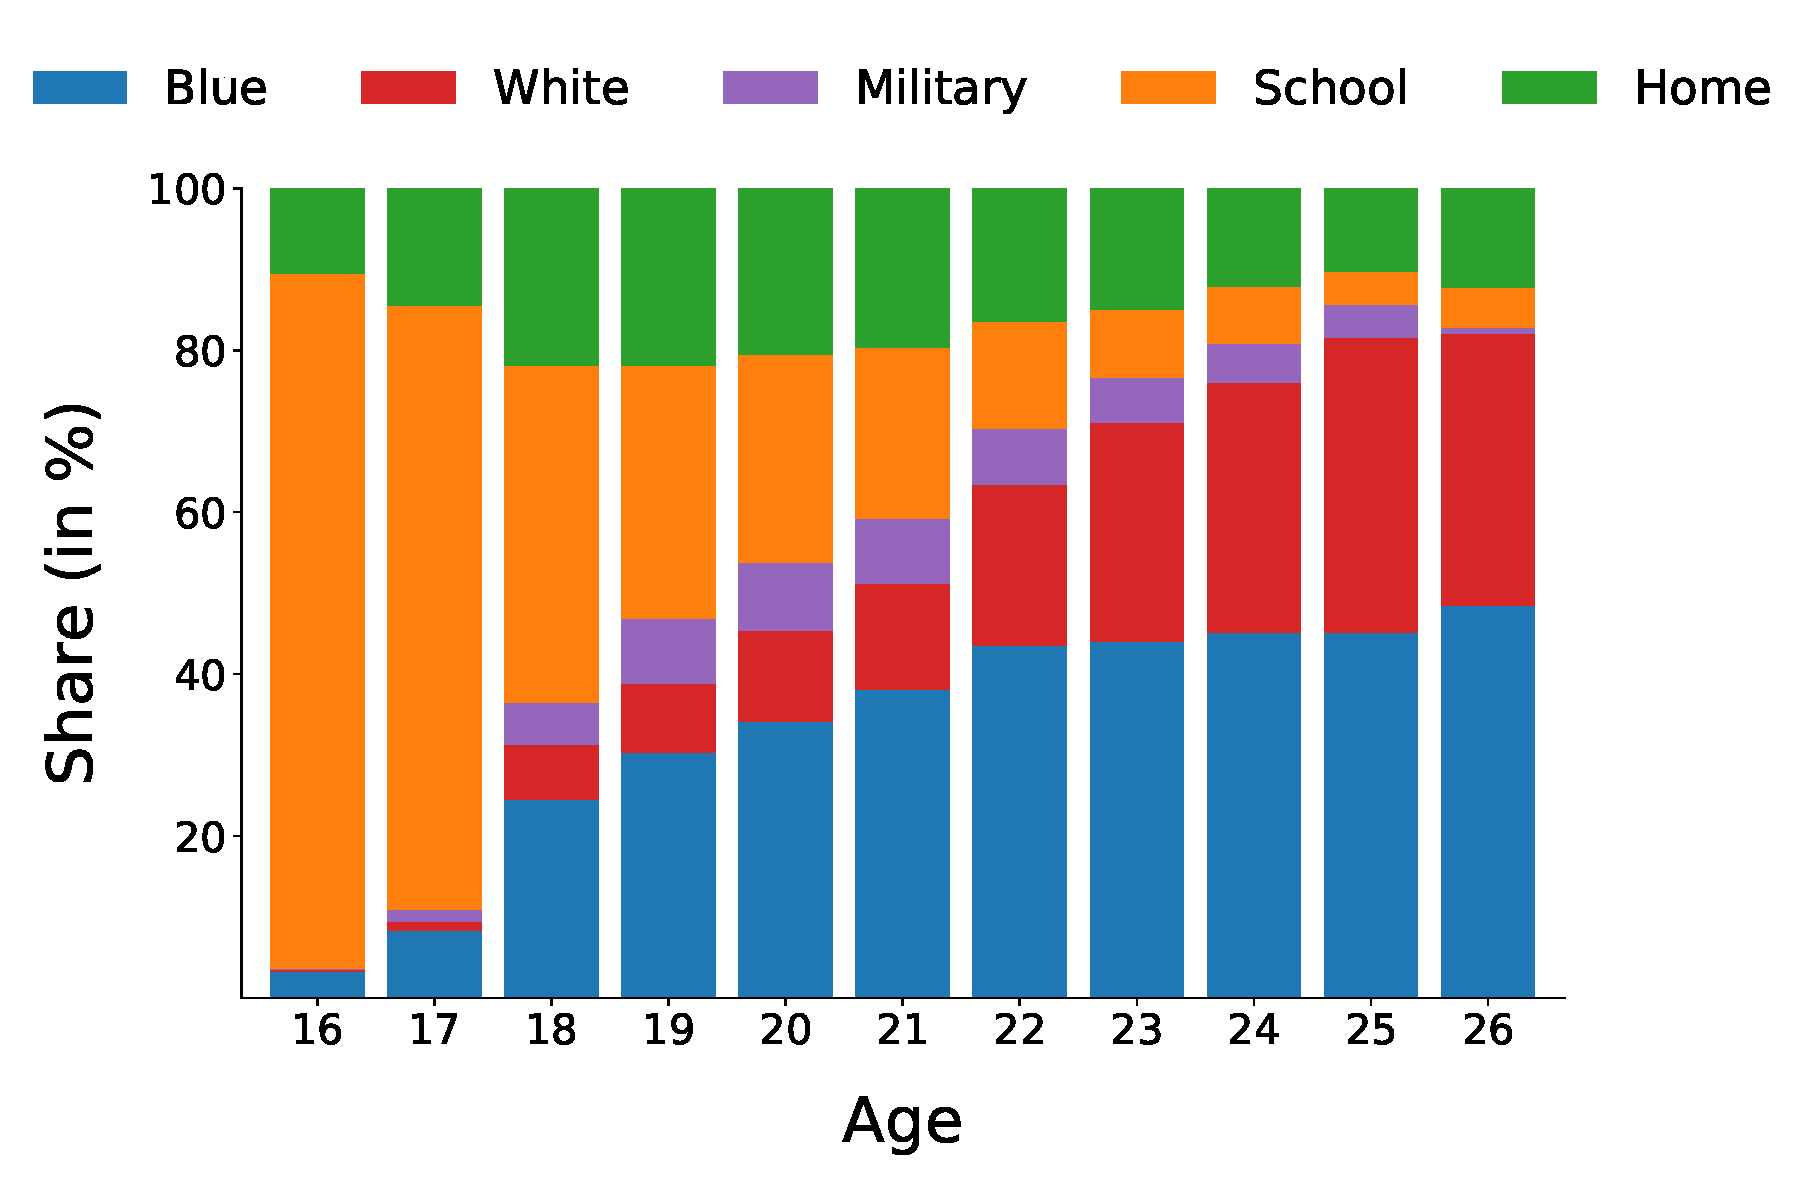
\includegraphics{fig-data-choice-all}}
  \end{figure}
\end{frame}

%-------------------------------------------------------------------------------
%-------------------------------------------------------------------------------
\begin{frame}
  \begin{figure}
  \caption{Average wage}
  \scalebox{0.35}{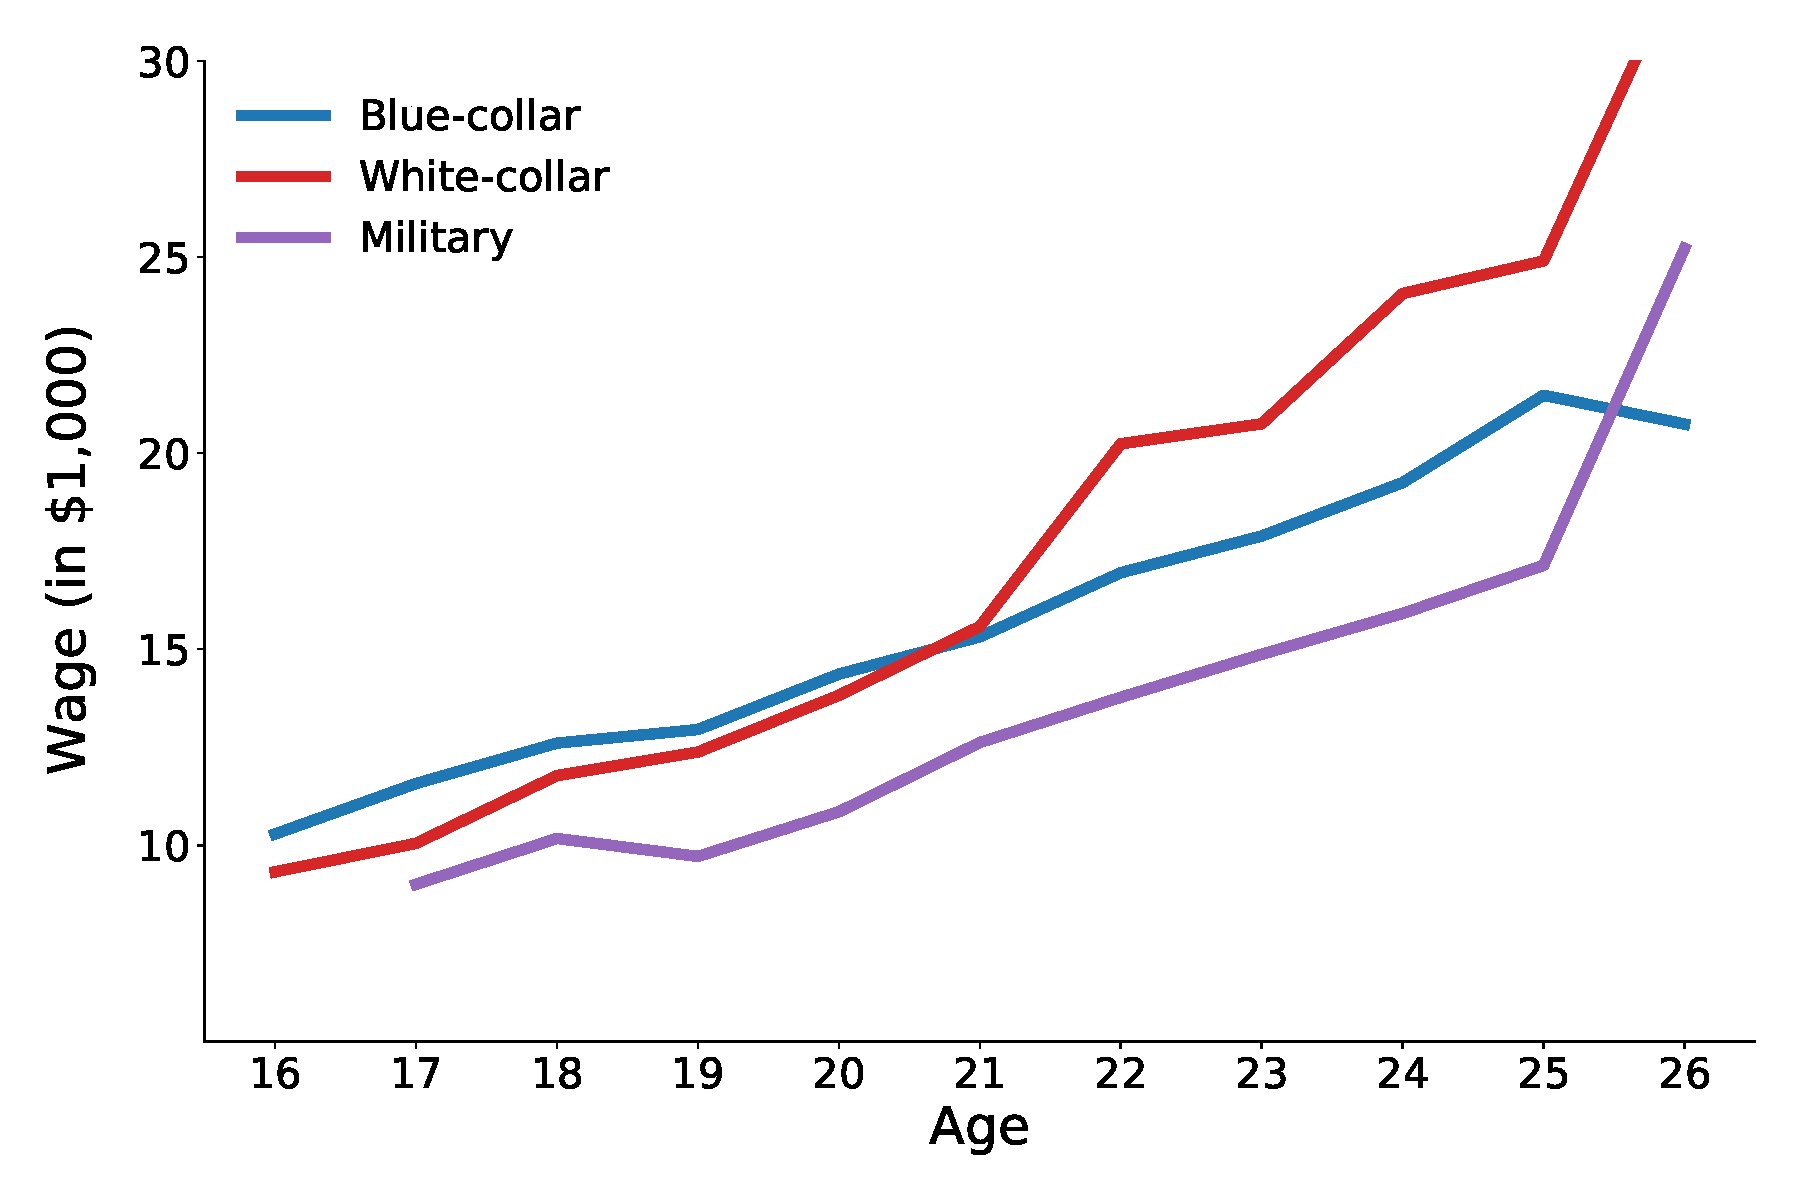
\includegraphics{fig-data-wage-occupations}}
  \end{figure}
\end{frame}
%-------------------------------------------------------------------------------
%-------------------------------------------------------------------------------
\begin{frame}\begin{center}
		\LARGE\textit{Economic insights}
\end{center}\end{frame}
%-------------------------------------------------------------------------------
%-------------------------------------------------------------------------------
\begin{frame}
  \begin{figure}[h!]\centering
  \caption{Economic mechanism and policy forecast}\label{Economic mechanism and policy forecast}
  \subfloat[Time preference]{\scalebox{0.175}{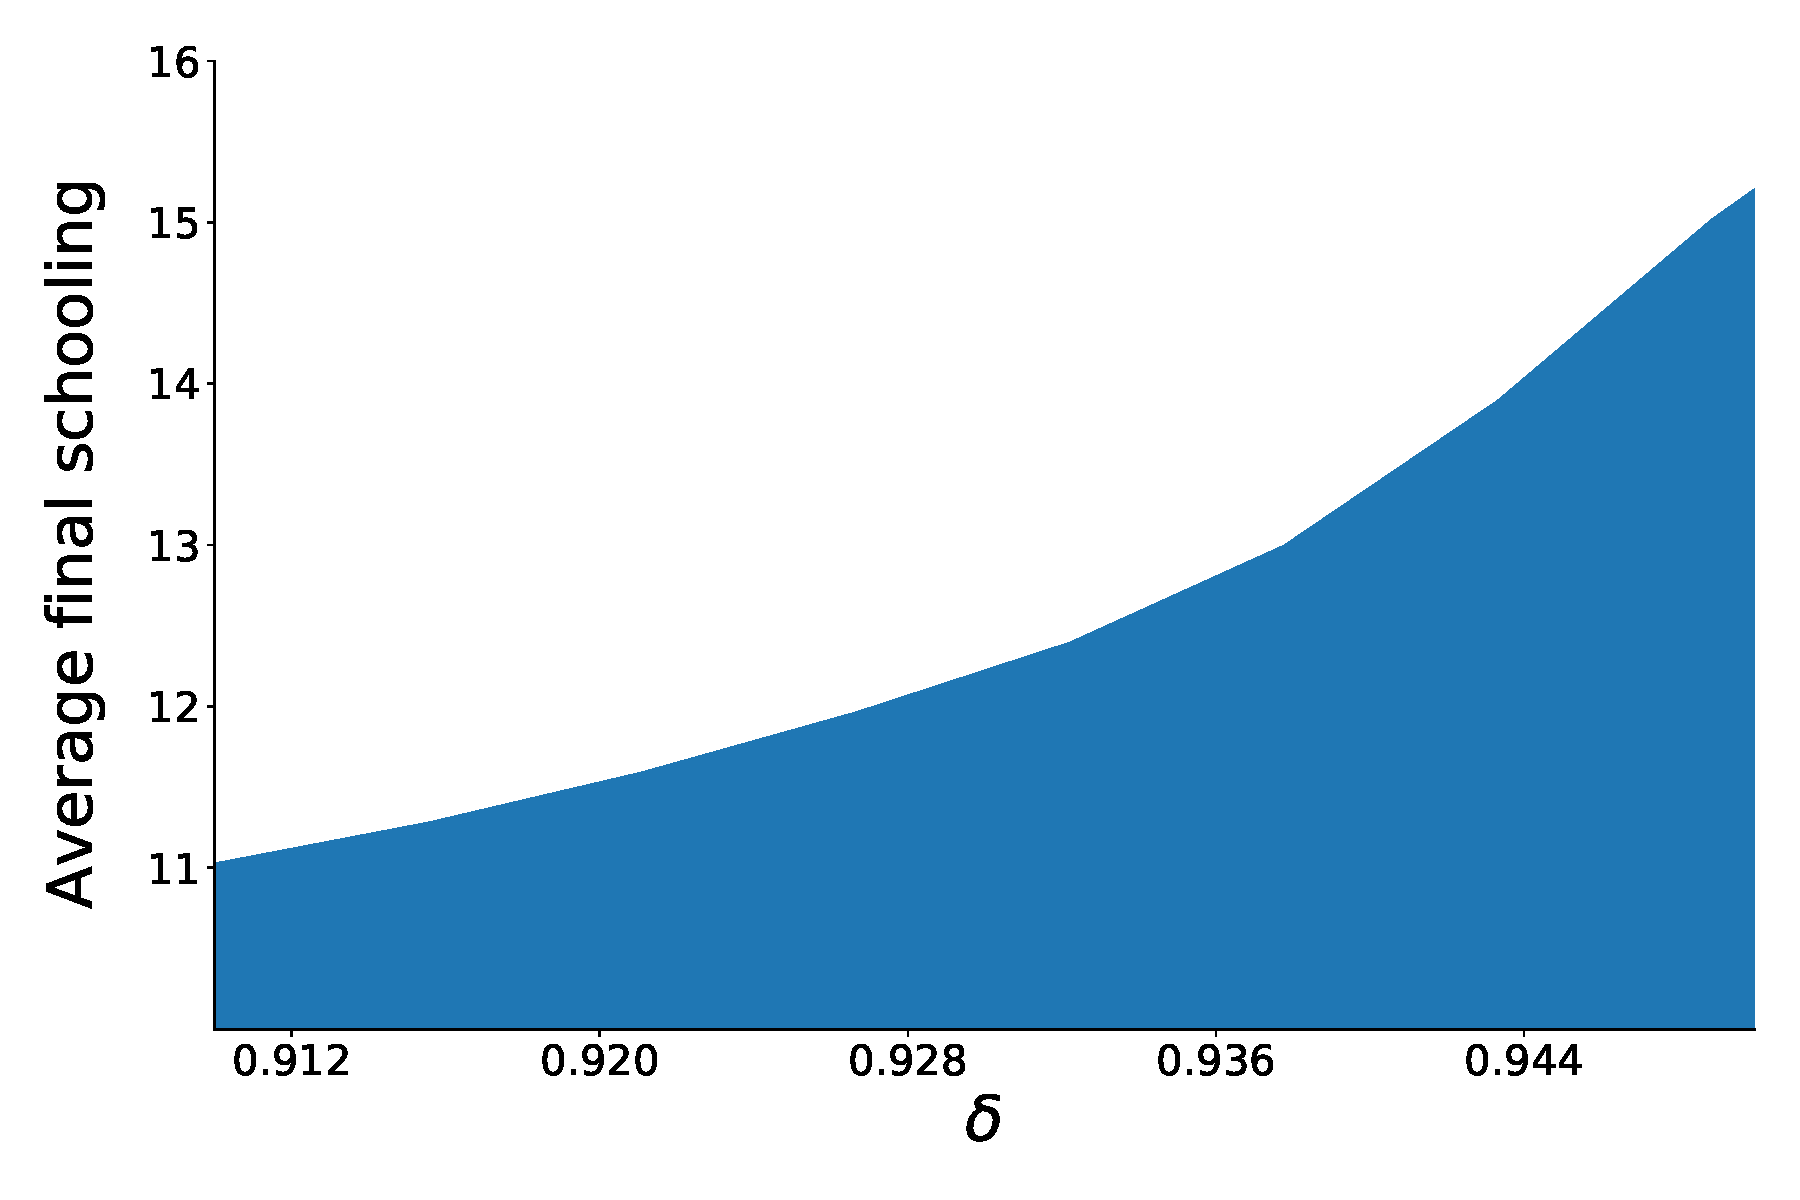
\includegraphics{fig-economic-mechanism}}}\hspace{0.3cm}
  \subfloat[Tuition subsidy]{\scalebox{0.175}{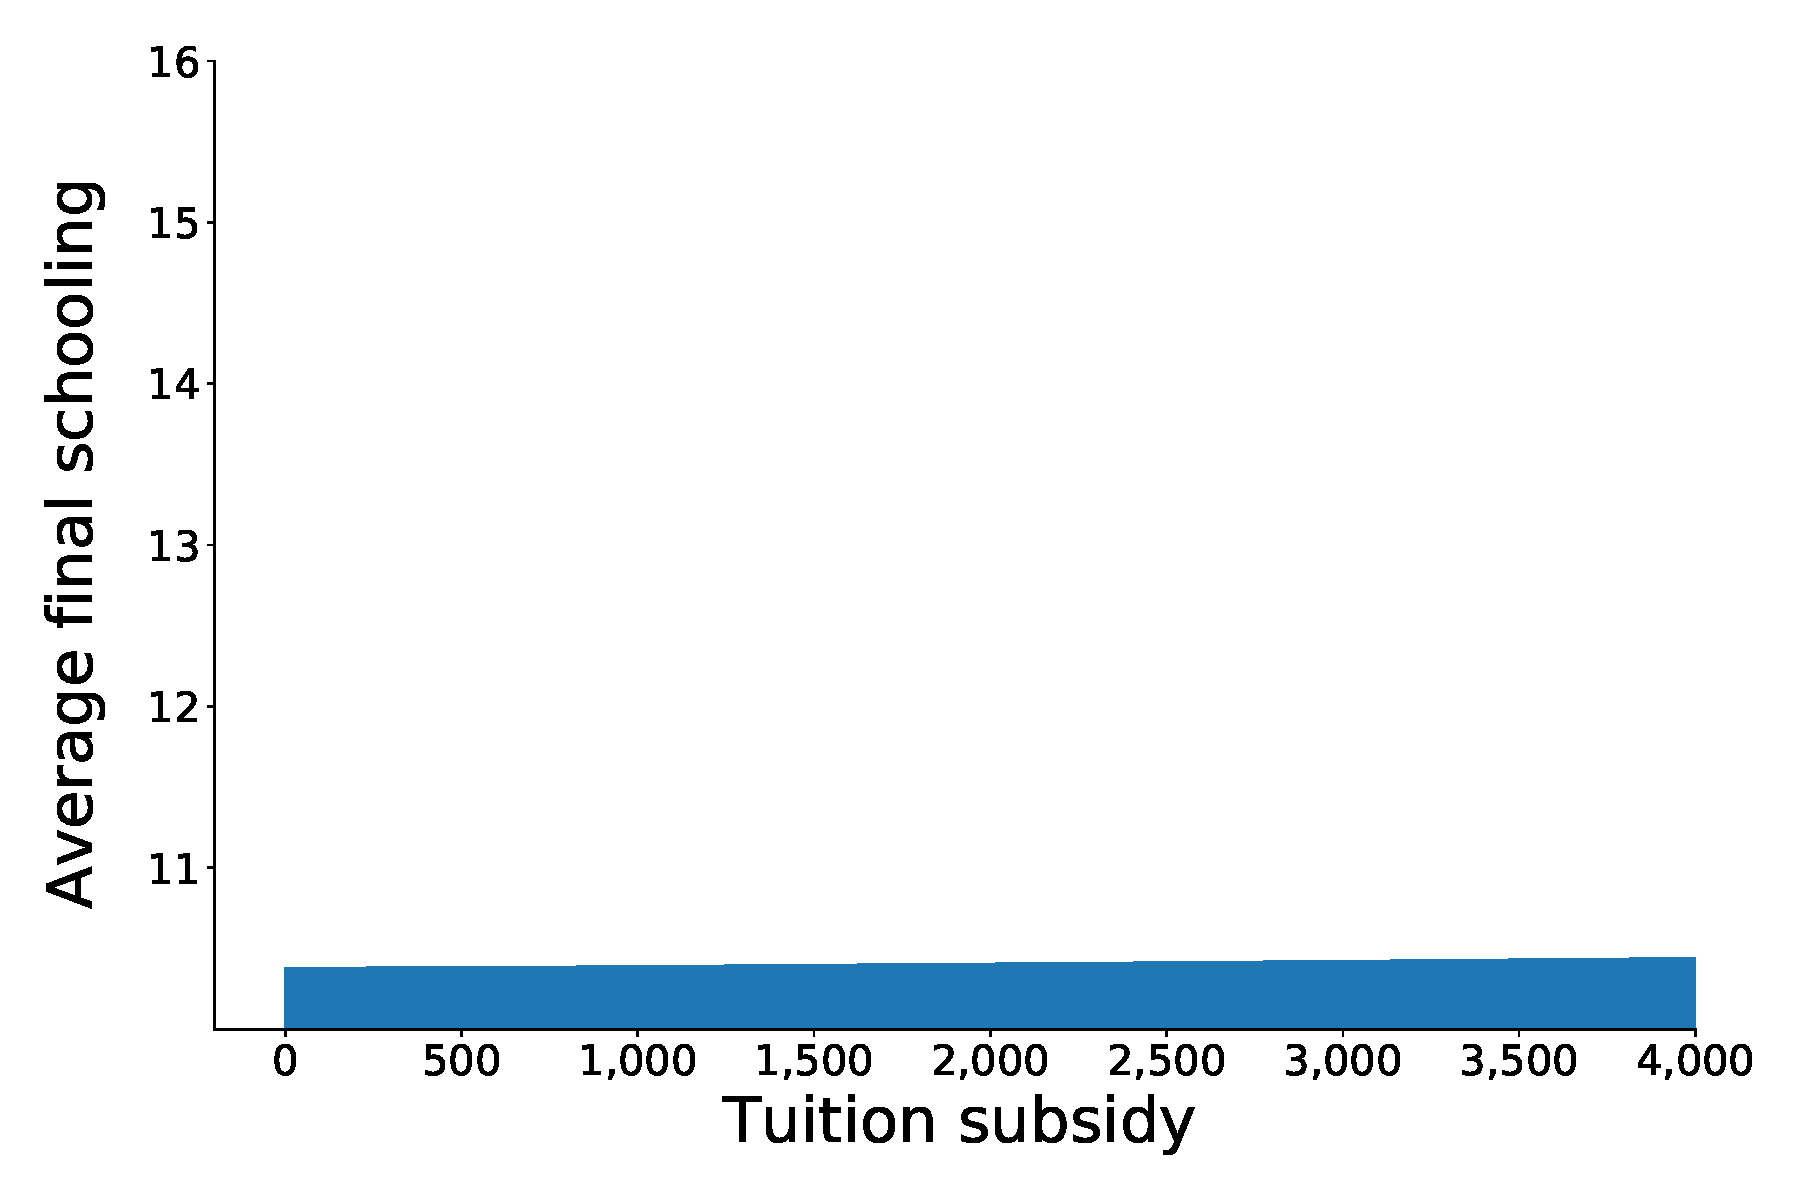
\includegraphics{fig-policy-forecast}}}
  \end{figure}
\end{frame}
